\documentclass[11pt]{amsart}
\usepackage{geometry}                % See geometry.pdf to learn the layout options. There are lots.
\geometry{letterpaper}                   % ... or a4paper or a5paper or ... 
%\geometry{landscape}                % Activate for for rotated page geometry
%\usepackage[parfill]{parskip}    % Activate to begin paragraphs with an empty line rather than an indent
\usepackage{graphicx}
\usepackage{amssymb}
\usepackage{epstopdf}
\usepackage [autostyle, english = american]{csquotes}
\usepackage{hyperref}
\MakeOuterQuote{"}
\DeclareGraphicsRule{.tif}{png}{.png}{`convert #1 `dirname #1`/`basename #1 .tif`.png}

\title{Project 4: Estimating Pi Using Monte Carlo Methods}
%\author{Jessica Bartley}
%\date{}                                           % Activate to display a given date or no date

\begin{document}
\maketitle
%\section{}
%\subsection{}

In this project we are to consider a series of higher and higher dimensional spheres.  We will fill in these volumes by using a Monte Carlo process in which we generate coordinates (ordered pairs) via a random number generator.  We will then count the number of coordinates that fall within the volume and the number of coordinates that fall outside of the volume.  These counts will be used to estimate the value of $\pi$.  This process is illustrated pictorially for the 2 dimensional case at \url{http://en.wikipedia.org/wiki/File:Pi_30K.gif}
\newline

\begin{figure}[ht!]
\centering
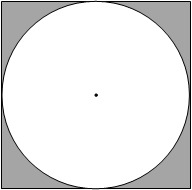
\includegraphics[width=40mm]{circle.jpg}
\caption{A sphere of dimension 2}
\label{overflow}
\end{figure}

Lets start with the familiar circle.  We need to accomplish the following:

\begin{enumerate}
\item Draw (or imagine drawing) a circle inscribed in a square. Lets say this circle has radius 1 and center at the origin.  Thus the areas are $A_{circle}=\pi$ and $A_{square}=4$.
\item Initiate counters $N_{hits}$ and $N_{total shots}$ at $0$.  Draw two random numbers $x$ and $y$ from a uniform distribution $P(x)=1$ where $x \in [0,1]$.  
\item Rescale these values so that $\textbf r =(2x-1,2y-1)$.  This ensures that they appear somewhere within the area of the square.
\item Increment the counters so that $N_{total shots}$ increases on each step and $N_{hits}=N_{hits}+1$ if $r^2 \leq 1$.
\item We stop this loop at some arbitrary value and analyze the estimator $\hat \pi = 4 \cdot \frac {N_{hits}} {N_{total shots}}$
\item Finally we analyze the error in our estimate via the variance: \newline $\sigma ^2 = 4^2 \cdot \frac{p (p-1)}{N_{totalshots}}$ where $p$ is the probability of making a hit, $p=\frac{A_{circle}}{A_{square}}$.
\end{enumerate}
\vspace{5 mm}

So now that we know how to do this in 2 dimensions, we need to write a code that will do this for $N=2...12$ dimensions.  What does a 12 dimensional sphere look like, you ask?  The answer is I have no idea.  But fortunately it doesn't matter.  What matters is that we have a formula for calculating the volume of an N dimensional sphere.

\begin{equation}
V_{Nsphere} = \frac {\pi ^{N/2}} {\Gamma (N/2+1)}
\end{equation}
\vspace{5 mm}

Where $\Gamma$ is the gamma function and is defined by $\Gamma(n)=(n-1)!$ for positive integers $n$.  The formula for an $N$ dimensional cube is 

\begin{equation}
V_{Ncube}=2^N
\end{equation}
\vspace{5 mm}

Where the cube's length is 2.  We are to repeat this process for spheres up to dimension 12.  The general process of estimating $\pi$ in $N$ dimensions is

\begin{equation}
\hat \pi = 4 \left[ \frac{N_{hits}}{N_{totalshots}} \cdot \frac{1}{\Gamma(n/2+1)} \right] ^{2/n}
\end{equation}
\vspace{5 mm}

The variance for the estimate of $\pi$ in $N$ dimensions is 

\begin{equation}
\sigma ^2 = 4^2 \cdot \left( \frac{1}{\Gamma(n/2+1)} \right) ^{4/n} \cdot \frac{p (p-1)}{N_{totalshots}}
\end{equation}
\vspace{5 mm}

Where $p$ is the probability of making a hit, $p= \frac{V_{Nsphere}}{V_{Ncube}}$.

\end{document}  